
\documentclass[11pt]{article}
\usepackage[margin=1.0in]{geometry}
\usepackage{amsmath,amssymb,amsthm}
\usepackage{booktabs,graphicx,microtype,xcolor,mdframed,float}
\graphicspath{{../figures/}}
\usepackage[colorlinks=true,linkcolor=RoyalBlue,urlcolor=RoyalBlue]{hyperref}
\usepackage[shortlabels]{enumitem}
\definecolor{RoyalBlue}{HTML}{1F4E79}
\definecolor{BoxBG}{HTML}{F4F6F8}
\definecolor{WarnBG}{HTML}{FDF3E7}
\newtheorem{proposition}{Proposition}
\newtheorem{corollary}[proposition]{Corollary}
\theoremstyle{remark}\newtheorem*{remark}{Remark}
\newmdenv[backgroundcolor=BoxBG,linewidth=.7pt,linecolor=black!30,innertopmargin=8pt,
  innerbottommargin=8pt,skipabove=10pt,skipbelow=10pt]{resultbox}
\newmdenv[backgroundcolor=WarnBG,linewidth=.7pt,linecolor=orange!55,innertopmargin=8pt,
  innerbottommargin=8pt,skipabove=10pt,skipbelow=10pt]{warnbox}
\newcommand{\Sa}{S_a}\newcommand{\Sb}{S_b}\newcommand{\Amax}{G_a^{\max}}\newcommand{\Bmax}{G_b^{\max}}

\title{\bfseries Nash Bargaining for Wholesaler Territory Division\\[2pt]
\large A discrete formulation over postal codes}
\author{}\date{}
\begin{document}\maketitle\vspace{-2.2em}

\begin{abstract}
\noindent Two merging wholesaling forces must divide a common territory. We formulate
the problem directly over postal codes and solve it by Nash bargaining from the zero
disagreement point: neither wholesaler can unilaterally revert to a pre-merger book once
the merger is executed, so the outside option is nothing, not the legacy territory.
Ordering zips by the ratio of the two wholesalers' utilities
gives a fast heuristic and, via outer approximation on the concave log-objective, an
exact solution with an optimality certificate. Nash is Pareto efficient
by construction, satisfies envy-freeness up to one zip, and cannot purchase fairness by
making both parties worse off --- a failure mode the equalisation criteria do exhibit.
Contiguity is then imposed exactly by a districting integer program --- solved by outer
approximation, since the log of the Nash product is concave rather than linear --- and
costs under half a percent of the bargaining product. A fifty-zip instance is worked through in full: allocation,
contiguity, contestability triage, and exact parameter breakpoints. Alternative
solution concepts and the constructions specific to them are collected in the
appendices.
\end{abstract}

\section{Setup}\label{sec:setup}
Index postal codes $z=1,\dots,n$, each carrying pre-merger sales $A_z$ to wholesaler $a$
and $B_z$ to wholesaler $b$, and total market opportunity $M_z$ (demand net of what
either has already written); write $M=\sum_zM_z$. Two parameters govern how a zip's
value splits between whichever wholesaler is assigned it and whichever is not.
\emph{Transfer capture} $\theta\in[0,1]$ is the share of a book the non-incumbent retains
after taking over the zip --- attrition and persistency account for $1-\theta$.
\emph{Headroom credit} $\lambda\in[0,1]$ is how much a dollar of unwritten opportunity
counts against a dollar of booked production.

Headroom is taken \emph{net}: whoever is assigned $z$ is credited with opportunity net of
business already on the books there, not gross of it. Gross double-counts and is
incoherent whenever $\lambda>\theta$ --- it would make an inherited book of business a
\emph{liability}, since the same dollar of production is worth more credited as headroom
than credited as a captured book. Under the net convention, with
\begin{equation}\label{eq:coefs}
c_1=1-\lambda,\qquad c_2=\theta(1-\lambda),
\end{equation}
the value of zip $z$ to each wholesaler, were it assigned the whole territory, is
\begin{equation}\label{eq:util}
u_a(z)=c_1A_z+c_2B_z+\lambda M_z,\qquad u_b(z)=c_2A_z+c_1B_z+\lambda M_z .
\end{equation}
$u_a$ credits wholesaler $a$ with all of their own book, a $\theta$-share of $b$'s, and a
$\lambda$-share of what neither has written; $u_b$ is the mirror image. Net headroom is
feasible only if it is non-negative pointwise,
\begin{equation}\label{eq:headroom}
M_z\ \ge\ \max\bigl(A_z+\theta B_z,\ B_z+\theta A_z\bigr)\qquad\text{for every }z,
\end{equation}
which we take as maintained throughout. An \emph{allocation} is a partition of
$Z=\{1,\dots,n\}$ into a set $S$ given to wholesaler $a$ and its complement
$Z\setminus S$ given to $b$: every zip is assigned, to exactly one side, with no third
disposition.

\section{The bargaining problem}\label{sec:statement}

This section poses territory division as a two-person bargaining problem in the classical
sense (Nash 1950), then works down from that object to the program actually solved.
Seven layers.

\subsection{Layer 1 --- players, outcomes, and the feasible set}
The players are the two wholesalers, $a$ and $b$. An outcome is an allocation $S\subseteq
Z$ as defined above, giving each player the payoff
\begin{equation}\label{eq:payoffs}
U_a(S)=\sum_{z\in S}u_a(z),\qquad U_b(S)=\sum_{z\notin S}u_b(z),
\end{equation}
using the utilities \eqref{eq:util}. The \emph{feasible set}
\begin{equation}
F=\bigl\{\bigl(U_a(S),\,U_b(S)\bigr)\ :\ S\subseteq Z\bigr\}\ \subset\ \mathbb{R}^2
\end{equation}
is the set of attainable payoff pairs: a cloud of at most $2^n$ points, entirely
determined by the data $(A_z,B_z,M_z)$ and the parameters $\theta,\lambda$.

\subsection{Layer 2 --- the disagreement point}
A bargaining problem is a pair $(F,d)$, where $d\in\mathbb{R}^2$ is the
\emph{disagreement point}: the payoff each player secures unilaterally, without the
other's cooperation, if no allocation is agreed. Getting $d$ right is not a normalisation
--- it is a claim about what each wholesaler can actually walk away with, and it is the
single most consequential modelling choice in this paper.

An earlier draft set $d=(\Sa,\Sb)$, each wholesaler's pre-merger production: if the
division fails, each keeps the book they walked in with. This is the natural first guess,
and it is wrong. A disagreement point must be an outcome a player can execute
\emph{unilaterally} if bargaining breaks down. Once the merger closes, pre-merger
production is not such an outcome: the separate sales forces, appointments, and client
relationships that generated $\Sa$ and $\Sb$ are dissolved into the merged entity, and
neither wholesaler can unilaterally resurrect them regardless of how the territory
dispute resolves. $\Sa$ is a historical number, not a threat point. What each wholesaler
can secure by failing to agree is nothing: absent an assignment, neither is appointed or
staffed to write business anywhere in the disputed territory. The disagreement point is
therefore the origin,
\begin{equation}\label{eq:dpoint}
d=(0,0).
\end{equation}

\begin{warnbox}
\textbf{This is not a matter of taste.} $d=(\Sa,\Sb)$ with $\Sa\ne\Sb$ is not a neutral
rescaling: bargaining from an asymmetric threat point is observationally equivalent to
an \emph{asymmetric} Nash solution at $d=0$ with an implicit, undisclosed weight (here
$\omega\approx0.54$ on the worked instance) --- a tilt toward whichever side had the
bigger pre-merger book, smuggled in through the disagreement point rather than argued for
on its merits. It also forfeits envy-freeness up to one good (EF1): the Nash bargaining
solution is EF1 \emph{at $d=0$} (Caragiannis et al.\ 2019) and the guarantee does not
survive moving $d$ away from the origin. Both defects disappear at $d=(0,0)$.
\end{warnbox}

Writing $g_a(S)=U_a(S)-0$ and $g_b(S)=U_b(S)-0$ for the gains relative to $d$, gains are
simply bundle utilities:
\begin{equation}\label{eq:gains}
g_a(S)=\sum_{z\in S}u_a(z),\qquad g_b(S)=\sum_{z\notin S}u_b(z),\qquad
\Amax=\sum_zu_a(z),\qquad \Bmax=\sum_zu_b(z),
\end{equation}
with $\Amax,\Bmax$ the attainable maxima from receiving the whole territory. Because
$\theta,\lambda\in[0,1]$ and \eqref{eq:headroom} holds, $u_a(z),u_b(z)\ge0$ pointwise, so
$g_a(S)>0$ for every non-empty $S$ and $g_b(S)>0$ for every $S\ne Z$: unlike the
pre-merger baseline, where headroom below a threshold $\lambda^\ast$ left the bargaining
set empty, feasibility of both gains is automatic here for any non-trivial split. That
threshold was an artefact of the discarded convention and does not arise at $d=0$.

\subsection{Layer 3 --- Nash's axioms and the solution}
Nash (1950) shows that if $F$ is convex and compact and contains a point strictly
dominating $d$, exactly one point of $F$ satisfies four axioms:
\begin{description}[leftmargin=1.6em,itemsep=1pt]
\item[Pareto optimality.] No other feasible point makes both players weakly better off
  and one strictly better off.
\item[Symmetry.] If $F$ is symmetric in the two players and $d_a=d_b$, the solution gives
  them equal payoff.
\item[Invariance to affine transformations.] The solution commutes with independently
  rescaling and shifting either player's utility --- utility is cardinal only up to a
  positive affine transformation, and the solution must not depend on the choice of
  units.
\item[Independence of irrelevant alternatives.] Shrinking $F$ to a subset that still
  contains the solution does not change it.
\end{description}
That point is the maximiser of the \emph{Nash product}, the product of gains over the
disagreement point:
\begin{equation}\label{eq:nashprod}
\max_{(U_a,U_b)\in F}\ \bigl(U_a-d_a\bigr)\bigl(U_b-d_b\bigr)
\qquad\text{subject to } U_a>d_a,\ U_b>d_b .
\end{equation}
No other point of $F$ satisfies all four axioms simultaneously; this is what makes
\eqref{eq:nashprod} a characterisation rather than one criterion among several equally
defensible ones.

\begin{warnbox}
\textbf{$F$ is not convex here.} Nash's theorem is stated for convex, compact $F$; with
indivisible postal codes $F$ is a finite point cloud instead, so strictly the axioms
select a \emph{lottery} over two adjacent allocations, and \eqref{eq:nashprod} maximised
over the point cloud is the discrete analogue rather than the axiomatic solution itself.
The gap is quantified in the remark on convexity in Section~\ref{sec:exact}: $0.0034\%$
on the worked instance. Known, small, ignored in practice; worth re-checking on real
data.
\end{warnbox}

\subsection{Layer 4 --- specializing to the discrete allocation problem}
At $d=(0,0)$, applying \eqref{eq:nashprod} to the feasible set generated by allocations
gives the criterion actually solved throughout this paper:
\begin{equation}\label{eq:nashcriterion}
\max_{S\subseteq Z}\ g_a(S)\,g_b(S),\qquad g_a(S)>0,\ g_b(S)>0,
\end{equation}
with $g_a,g_b$ as in \eqref{eq:gains}. The remainder of this section turns
\eqref{eq:nashcriterion} into a program that can be handed to a solver: first restricting
$F$ by operational constraints (contiguity, state borders), then writing the result as a
mixed-integer program, then solving it exactly.

\subsection{Layer 5 --- constraints shrink $F$}
Operational requirements restrict which $S$ are admissible, and therefore which points of
$F$ are attainable. Contiguity --- each wholesaler receiving one connected territory on
the postal-code adjacency graph $G=(Z,E)$ --- is the binding one:
\begin{equation}
F_{\text{cont}}=\bigl\{(g_a(S),g_b(S))\ :\ G[S]\text{ and }G[Z\setminus S]\text{ both connected}\bigr\}\ \subseteq\ F .
\end{equation}
The same bargaining problem is then solved on the smaller set. \emph{That is the precise
game-theoretic content of the districting constraints: they do not change the criterion,
they shrink the feasible set.} State-border restrictions act identically, by deleting
cross-state edges from $G$ before connectivity is assessed.

\subsection{Layer 6 --- the program}
Maximising \eqref{eq:nashprod} over $F_{\text{cont}}$ at $d=(0,0)$, with
$x_z=\mathbf{1}[z\in S]$:
\begin{align}
\max_{x\in\{0,1\}^n}\quad & \log g_a+\log g_b \label{eq:obj}\\
\text{s.t.}\quad
& g_a=\sum_z x_z u_a(z), \qquad g_b=\sum_z (1-x_z)u_b(z), \label{eq:lin}\\
& g_a>0,\quad g_b>0, \label{eq:feas}\\
& G[S]\ \text{and}\ G[Z\setminus S]\ \text{connected}. \label{eq:conn}
\end{align}

\begin{resultbox}
\textbf{This is a convex MINLP.} The gains \eqref{eq:lin} are \emph{linear} in $x$; the
objective \eqref{eq:obj} is \emph{concave} in those linear expressions; connectivity
\eqref{eq:conn} is representable by linear constraints. Maximising a concave function
over a mixed-integer linear feasible set is the well-behaved MINLP class, for which
outer approximation is a finite global method. The product form
$\max g_ag_b$ is \emph{not} concave --- it is bilinear and indefinite --- so the
logarithm is not cosmetic: it is what places the problem in the tractable class.
\end{resultbox}

\subsection{Two representations of connectivity}
Constraint \eqref{eq:conn} is not a linear inequality as written. Two standard encodings.

\paragraph{(a) Compact, single-commodity flow.} Fix roots $r_a,r_b$. Introduce
$f^a_{uv}\ge0$ on each arc. Every zip assigned to $a$ absorbs one unit of flow sent from
$r_a$ through arcs internal to $a$'s territory:
\begin{align}
\sum_{(u,z)\in E} f^a_{uz}-\sum_{(z,v)\in E} f^a_{zv} &= x_z, && z\ne r_a,\\
f^a_{uv} &\le (n-1)\,x_u, \qquad f^a_{uv}\le (n-1)\,x_v, && (u,v)\in E,
\end{align}
with the mirror system in $(1-x)$ for $b$. Polynomial size, $O(|E|)$ continuous
variables per district, one solve.

\paragraph{(b) Exponential, separator cuts.} For every $S'\subseteq Z$ inducing a
component not containing the root,
\begin{equation}\label{eq:cut2}
|S'|\sum_{w\in N(S')}x_w\ \ge\ \sum_{v\in S'}x_v .
\end{equation}
There are exponentially many such inequalities, so they are generated \emph{lazily}: solve,
inspect the incumbent for disconnected components, add the violated cuts, re-solve. In
practice a handful of rounds suffice. This is the encoding used here; it keeps the model
small at the cost of repeated solves.

\subsection{Layer 7 --- solving it}
Outer approximation linearises the concave objective from above. Introduce
$z_a\le\log g_a$, $z_b\le\log g_b$ enforced by supporting hyperplanes \eqref{eq:tangent},
and maximise $z_a+z_b$. Each relaxation is a pure MILP; its optimum is an upper bound on
\eqref{eq:obj}; a tangent added at the incumbent tightens it. Interleaving the tangent
cuts with the connectivity cuts \eqref{eq:cut2} converges both simultaneously, and
termination when the incumbent's true log-product meets the bound is an optimality
\emph{certificate}. Compactness may be priced by subtracting
$\rho\sum_{e}y_e$ with $y_e\ge|x_u-x_v|$, at the cost of changing the objective.

\begin{center}
\begin{tabular}{clll}
\toprule
\textbf{layer} & \textbf{object} & \textbf{form}\\
\midrule
1 & players, outcomes, feasible set $F$ & $2^n$ points\\
2 & disagreement point & $d=(0,0)$\\
3 & Nash's axioms $\Rightarrow$ solution & $\max(U_a-d_a)(U_b-d_b)$\\
4 & discrete specialisation & $\max\,g_a(S)g_b(S)$\\
5 & constraints (contiguity, state borders) & shrink $F$\\
6 & program & \eqref{eq:obj}--\eqref{eq:conn}, convex MINLP\\
7 & method & outer approximation + lazy cuts, finite, certified\\
\bottomrule
\end{tabular}
\end{center}

\section{The Nash solution}\label{sec:nash}
Section~\ref{sec:statement} reduced fair division to the criterion
\eqref{eq:nashcriterion}, $\max_{S\subseteq Z}g_a(S)g_b(S)$ subject to $g_a,g_b>0$. This
section gives the exact algorithm. A fast, solver-free heuristic based on ordering zips
by exchange rate --- useful as a preview or sanity check, but not exact for Nash --- is
developed in Appendix~\ref{app:prefix}.

\label{sec:exact}
Taking logarithms, $\log(g_ag_b)=\log g_a+\log g_b$, does not linearise the objective:
$g_a$ is linear in $x$, so $\log g_a$ is \emph{concave} in a linear expression. The
problem is therefore a convex MINLP --- maximising a concave function over a
MILP-representable set --- for which outer approximation is a finite \emph{global}
method. Introduce $z_a\le\log g_a$ and add supporting hyperplanes
\begin{equation}\label{eq:tangent}
z_a\ \le\ \log(\hat g)+\frac{g_a-\hat g}{\hat g},
\end{equation}
one linear cut per tangent point, no additional binaries, and maximise $z_a+z_b$. The
tangent set is a relaxation, so the MILP optimum is a valid \emph{upper bound}; adding
a tangent at the incumbent and re-solving tightens it, and when the incumbent's true
log-product meets the bound the incumbent is globally optimal. This is a certificate,
not a stopping heuristic.

\begin{resultbox}
Validated against exhaustive enumeration, $120$ random instances per size: exact match
in $100\%$ of cases at every $n$ tested, with bound gap identically zero. Cost is $6$--$7$
iterations regardless of size --- $0.10$s at $n=50$, $0.84$s at $n=400$. \textbf{Use the
exact method by default}; the prefix table (Appendix~\ref{app:prefix}) is a fast preview
and a sanity check.
\end{resultbox}

\begin{remark}[Convexity, and what "Nash" means over indivisible zips]
Nash's axiomatic characterisation --- Pareto efficiency, symmetry, scale invariance,
independence of irrelevant alternatives --- assumes the bargaining set is
\emph{convex}. With indivisible postal codes the feasible set
$F=\{(g_a(S),g_b(S))\}$ is a finite point cloud, so strictly the axioms deliver a
\emph{lottery} over two adjacent allocations, and $\max g_ag_b$ over $F$ is the natural
discrete analogue rather than the axiomatic solution itself. The distinction is
quantitatively small here: the Nash product on the convex hull, where randomisation is
permitted, is $24.09177$ against $24.09096$ for the best deterministic allocation --- a
difference of $0.0034\%$. The frontier is dense enough that the deterministic vertex
lies essentially on the hull. It is worth re-checking on real data, and not worth
randomising territory assignments over.
\end{remark}

\begin{remark}[No fixed point is needed]
In a continuum the Nash threshold satisfies $t^\star=g_a/g_b$, a fixed point whose
naive iteration diverges --- on this instance it runs
$1.000\to40.22\to-0.244\to-6.447$ into a degenerate corner. Neither the prefix table nor
the outer approximation requires it.
\end{remark}

\section{Why Nash}\label{sec:why}
\paragraph{Exactly solvable.} Outer approximation (Section~\ref{sec:exact}) reaches a
certified global optimum in $6$--$7$ iterations regardless of $n$. The equalisation
criteria require search for their exact optima and carry no such certificate.

\paragraph{Pareto efficient by construction.} Maximising a product cannot be improved
for both parties simultaneously. The min-$|$difference$|$ criteria carry no such
guarantee and do fail in practice: an unconstrained equalising program reached a gap of
$0.000161$ while giving up $18\%$ of attainable welfare (Appendix~\ref{app:other}).

\paragraph{Envy-freeness up to one zip.} Neither wholesaler prefers the other's
territory once a single zip is removed from it --- the strongest fairness guarantee
available for indivisible goods, and legible in a room.

\paragraph{The one limitation.} Nash requires $g_a,g_b>0$, so below the feasibility
threshold $\lambda^\ast$ the bargaining set is empty. Report $\lambda^\ast$ explicitly;
under the net convention it was $0.069$ on the instances tested, well below any
defensible $\lambda$. Below it the merger is negative-sum for the wholesalers and the
conversation is not about criteria. The egalitarian criterion is the fallback there.

\paragraph{If seniority should count.} Asymmetric Nash,
$\max g_a^{\omega}g_b^{1-\omega}$, retains the prefix property with threshold
$\tfrac{1-\omega}{\omega}\cdot\tfrac{g_a}{g_b}$. An explicit weight is preferable to a
criterion that encodes a tilt nobody selected.

\section{A fifty-zip instance}\label{sec:instance}
Fifty postal codes on the unit square drawn from a two-component Gaussian mixture, with
metros at $(0.28,0.62)$ and $(0.72,0.36)$; $a$ is anchored on the first, $b$ on the
second, both present in each. Totals $\Sa=3.0$, $\Sb=1.8$, $M=40$ ($12\%$ combined
penetration); $\theta=0.4$, $\lambda=0.3$.

\begin{center}\begin{tabular}{lr}\toprule
$\mathrm{corr}(A_z,B_z)$ across zips & $+0.685$\\
utility ratio range & $[0.9531,\ 1.1373]$\\
minimum net headroom & $0.2335$\\
\bottomrule\end{tabular}\end{center}

\noindent The positive correlation is the harder configuration: both wholesalers are
strong in the same places. The ratio spans a narrow band mostly above $1$, so on raw
utility $a$ is favoured nearly everywhere and fairness is the only force conceding
territory to $b$.

\begin{figure}[H]\centering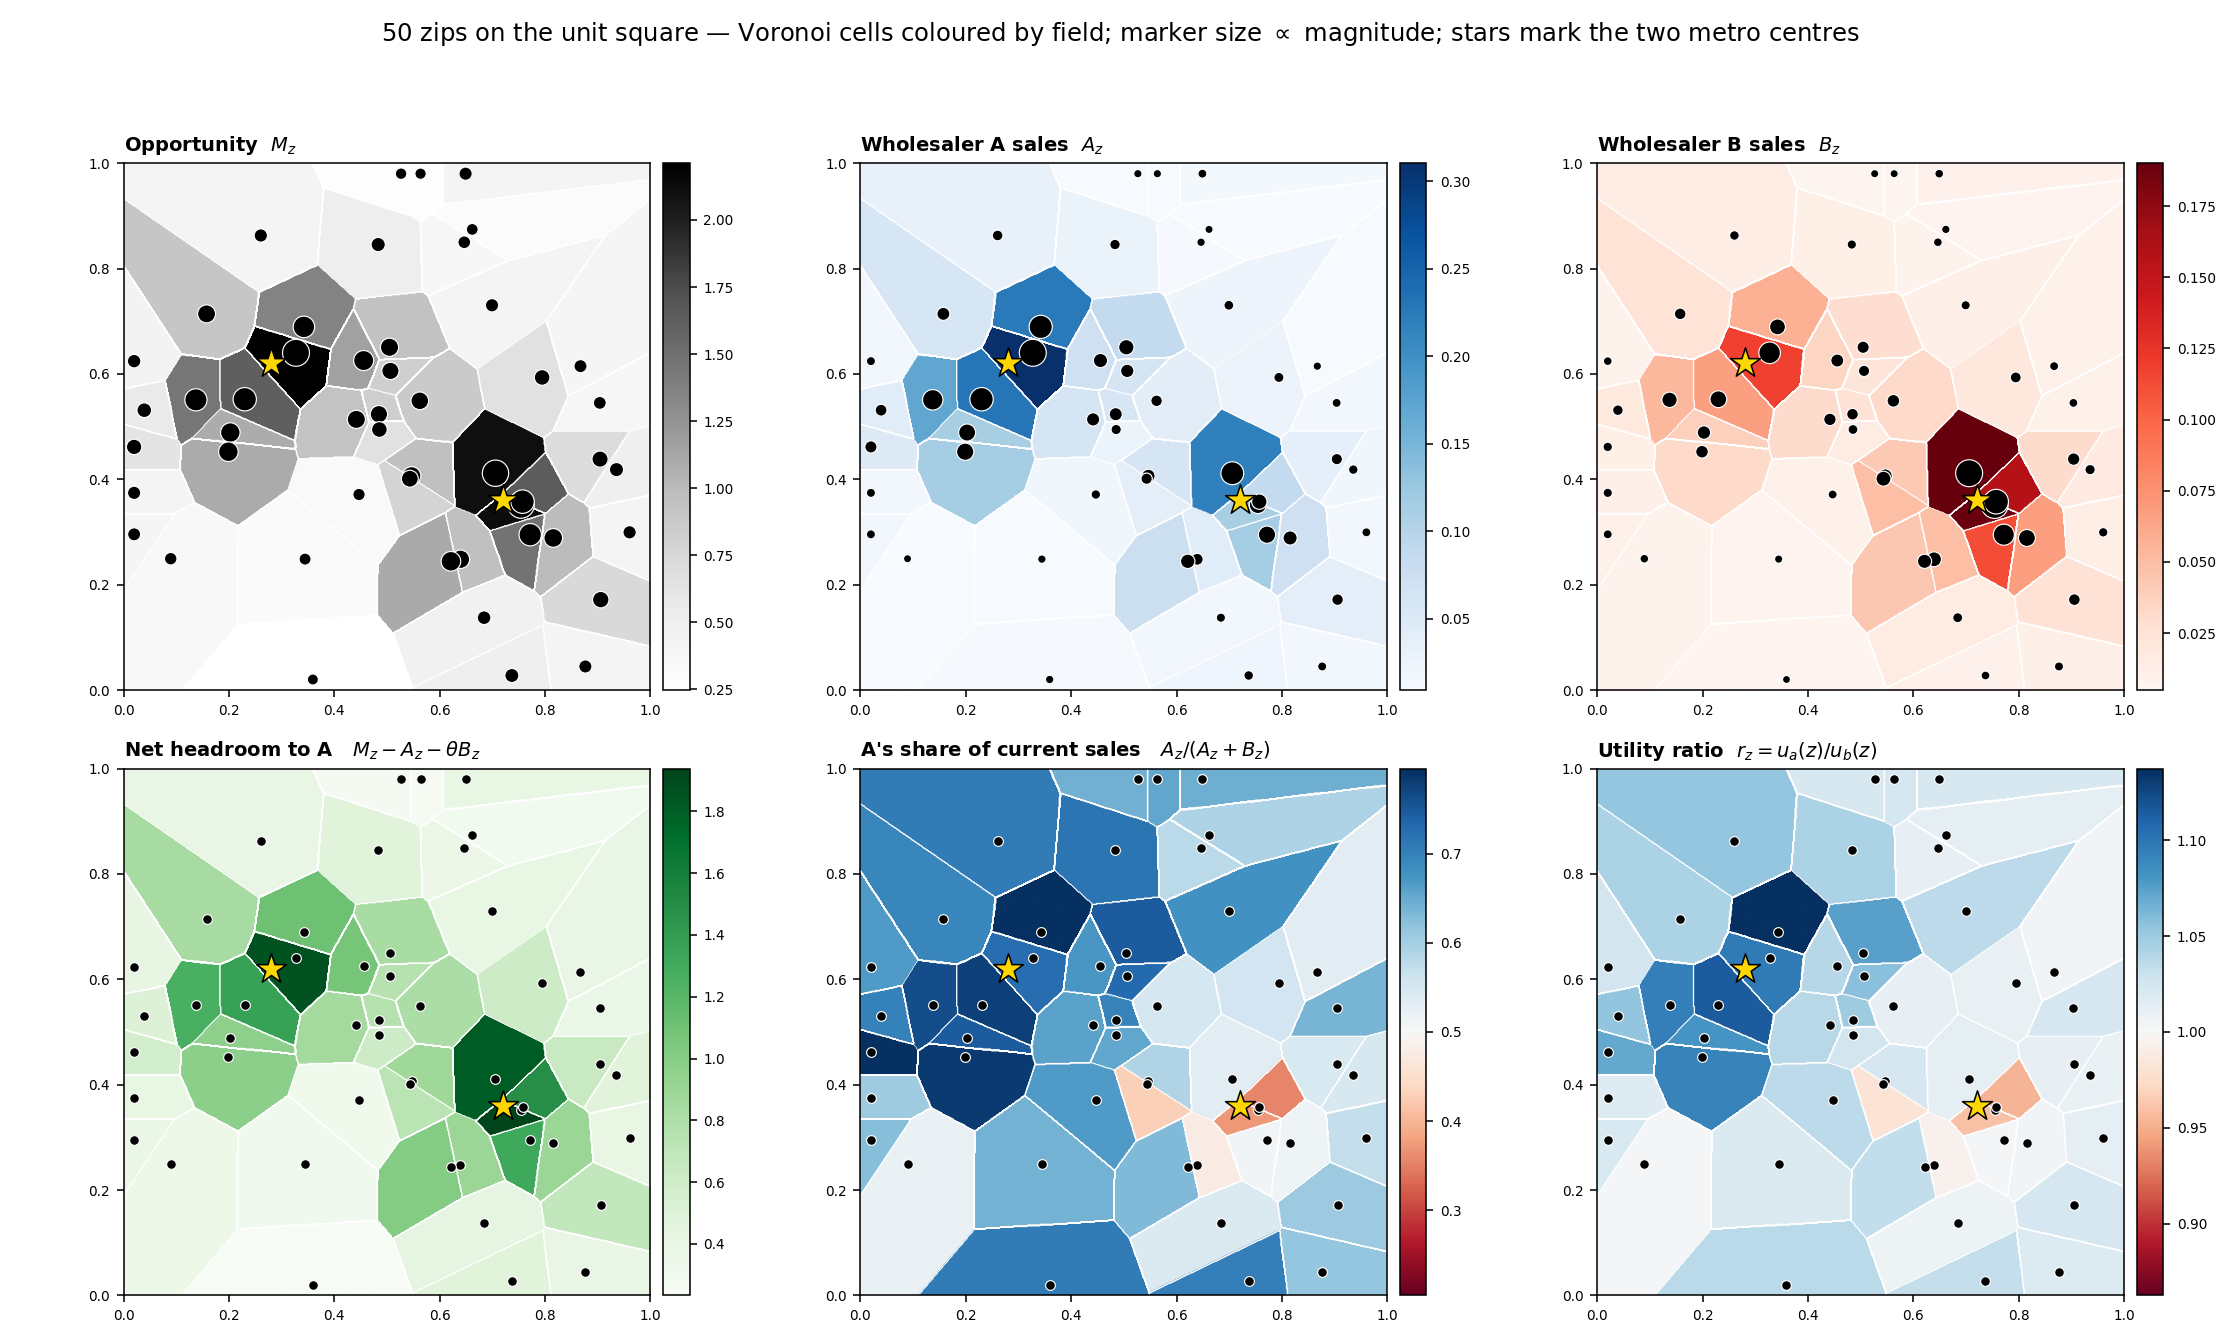
\includegraphics[width=\textwidth]{zip50_distributions.png}
\caption{The instance before optimisation. Voronoi cells coloured by field, marker size
proportional to magnitude, stars at metro centres.}\end{figure}

\subsection{Solution}
\begin{center}\begin{tabular}{lrrrr}\toprule
& $k$ & $g_a$ & $g_b$ & $g_ag_b$\\ \midrule
Nash, exact (outer approximation) & $25$ & $4.9787$ & $4.8388$ & $\mathbf{24.09117}$\\
Nash, prefix heuristic (Appendix~\ref{app:prefix}) & $25$ & $4.9360$ & $4.8807$ & $24.09096$\\ \bottomrule
\end{tabular}\end{center}

\noindent The two select \emph{different} allocations of the same size; the heuristic's
shortfall is $8.4\times10^{-6}$, which is negligible here but not zero.

\noindent $a$ receives $25$ zips, $53.1\%$ of opportunity. Equal gain and the
egalitarian criterion select the same allocation; Kalai--Smorodinsky differs by one zip
(Appendix~\ref{app:other}).

\begin{figure}[H]\centering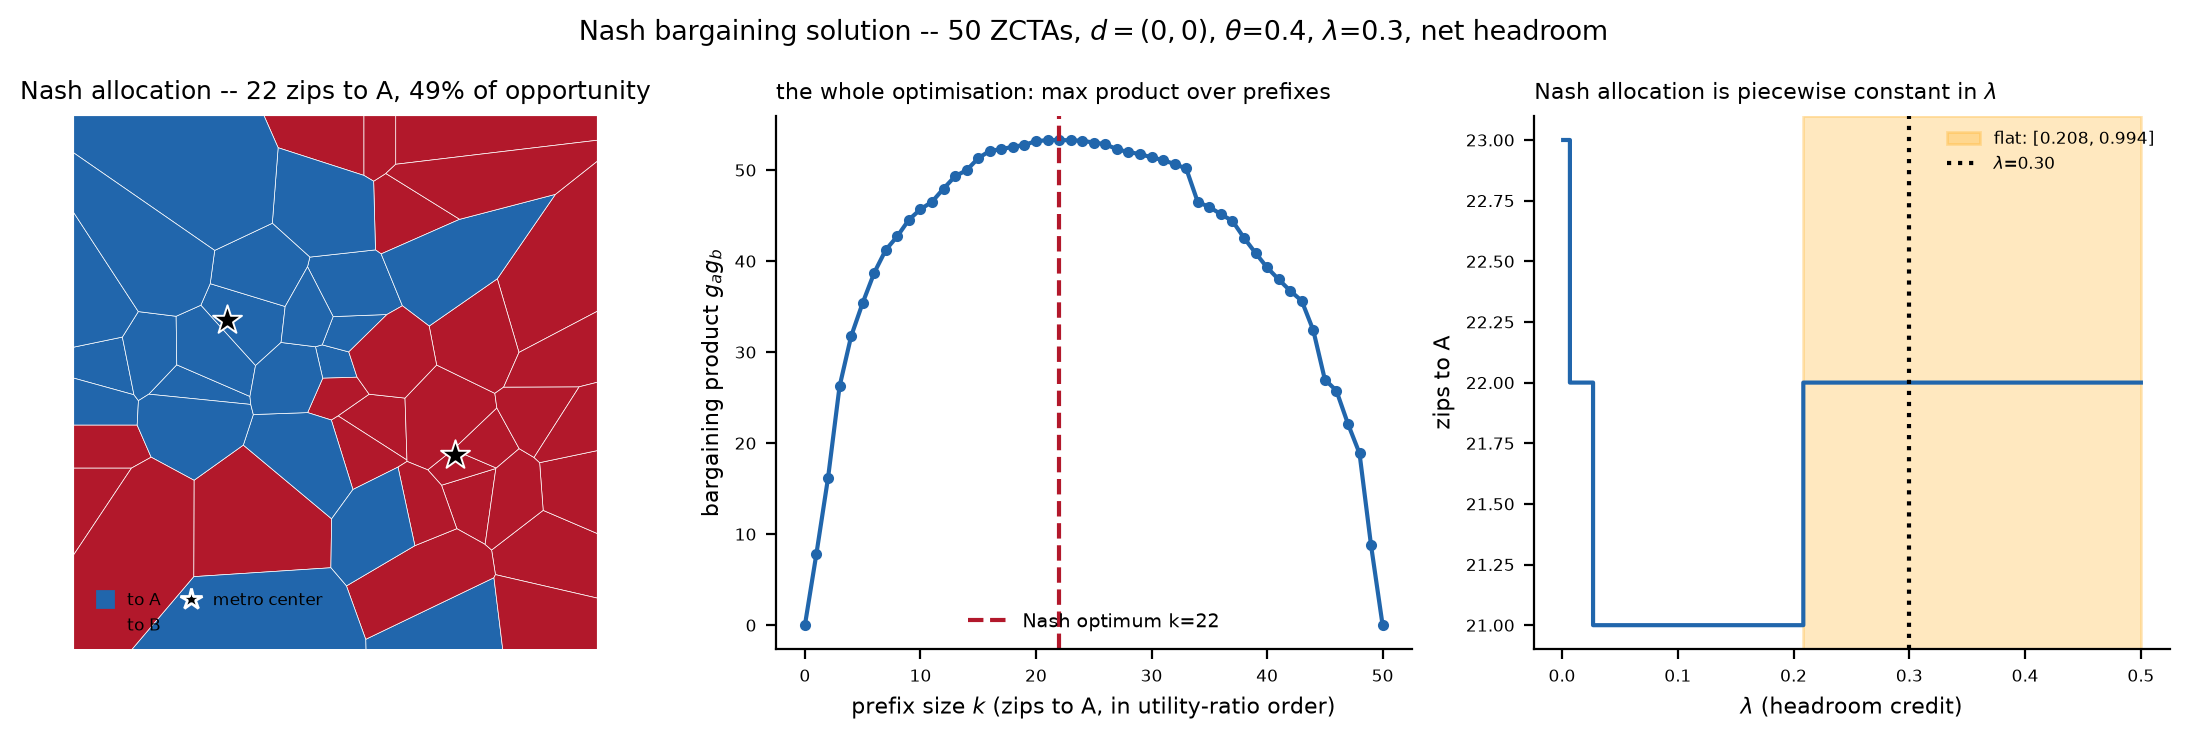
\includegraphics[width=\textwidth]{nash_solution.png}
\caption{Left: the Nash allocation. Centre: the entire optimisation --- the bargaining
product over the $n+1$ prefixes, maximised at $k=25$. Right: the allocation is
piecewise constant in $\lambda$, with $\lambda=0.30$ inside a flat interval running
from $0.265$ to $0.506$.}\end{figure}

\section{Contiguity}\label{sec:contig}
Nothing above forces each territory to be connected, and the Nash allocation is not:
$a$ holds two pieces and $b$ three, in each case a stray single zip. Imposing
connectivity turns the problem into a \emph{districting} integer program --- the
formulation used for electoral redistricting and sales-territory alignment --- with one
binary per zip.

\subsection{Formulation: the log makes it concave, not linear}
Taking logarithms separates the Nash product, $\log(g_ag_b)=\log g_a+\log g_b$, but does
not linearise it: $g_a$ is linear in $x$, so $\log g_a$ is \emph{concave} in a linear
expression. That is the useful case. A concave function is the lower envelope of its
tangents, so introduce $z_a\le\log g_a$ and add supporting cuts
\begin{equation}\label{eq:tangent}
z_a\ \le\ \log(\hat g)+\frac{g_a-\hat g}{\hat g},
\end{equation}
one linear constraint per tangent point $\hat g$, with no additional binaries. The
program is then
\begin{align}
\text{decision}\quad & x_z\in\{0,1\},\ 1 \text{ if } z\to a,\\
\text{objective}\quad & \max\ z_a+z_b-\rho\textstyle\sum_{e\in E}y_e,
\qquad y_e\ \ge\ |x_u-x_v| ,
\end{align}
with $z_a,z_b$ bounded by tangent cuts \eqref{eq:tangent}. The tangent set is an
\emph{outer} approximation --- an upper bound --- which tightens as tangents are added
at the incumbent solution. This is Kelley's cutting-plane method, and it interleaves
naturally with the contiguity cuts of Section~\ref{sec:cuts}: both converge together,
typically in about five iterations.

The $y_e$ count \emph{boundary edges}, the perimeter of the partition, and $\rho$
prices compactness. Note that $\rho>0$ \emph{changes the objective}: the solve is then
exact for Nash-minus-a-perimeter-penalty, a legitimate modelling choice but not exact
Nash. Set $\rho=0$ for the latter.

\begin{warnbox}
\textbf{Two traps.} First, the compactness term is not optional: fairness alone is
degenerate, many allocations achieve near-identical objective values, and contiguity
cuts never bite --- an implementation without it thrashed for seventeen rounds without
converging. Second, a weighted-sum scalarisation $wg_a+(1-w)g_b$ collapses to corner
solutions when the frontier is close to linear, as it is here, and an
$\varepsilon$-constraint sweep needs one MILP solve per frontier point. Outer
approximation avoids both, at roughly a twentieth of the cost.
\end{warnbox}

\subsection{Contiguity by separator cuts}\label{sec:cuts}
Fix a root zip per side. If $a$'s territory splits, then for each component $S$ not
containing $a$'s root add
\begin{equation}\label{eq:cut}
|S|\sum_{w\in N(S)}x_w\ \ge\ \sum_{v\in S}x_v ,
\end{equation}
``if any of $S$ is with $a$, some neighbour just outside must be too''; symmetric in
$(1-x)$ for $b$. Re-solve and repeat. The alternative is a single-commodity \emph{flow}
formulation --- ship one unit from each assigned zip to its root along in-district
edges --- exact in one solve but requiring $O(|E|)$ extra continuous variables per
district. Aggregating one cut per island rather than one per zip matters for
convergence.

\subsection{Result}
The exact unconstrained Nash allocation leaves $a$ in three pieces and $b$ in two, in
each case a stray single zip. Enforcing connectivity, and sweeping the compactness weight on
a graph of $50$ zips and $132$ adjacency edges:

\begin{center}\begin{tabular}{lrrrrrl}\toprule
$\rho$ & $g_ag_b$ & perimeter & \% of edges & iterations & time & pieces $a/b$\\ \midrule
--- (unconstrained) & $24.0910$ & --- & --- & --- & --- & $2/3$\\
$2\times10^{-3}$ & $24.0146$ & $15$ & $11.4\%$ & $5$ & $0.7$s & $1/1$\\
$2\times10^{-4}$ & $24.0569$ & $18$ & $13.6\%$ & $5$ & $0.1$s & $1/1$\\
$1\times10^{-5}$ & $24.0774$ & $33$ & $25.0\%$ & $10$ & $0.4$s & $1/1$\\
\bottomrule\end{tabular}\end{center}

\begin{resultbox}
The price of contiguity under Nash is between $0.06\%$ and $0.32\%$ of the bargaining
product, depending on how clean a boundary is wanted. Contiguity is close to free when
solved exactly. A greedy island-repair heuristic, by contrast, degraded the objective by
more than three orders of magnitude and should be used only to \emph{detect}
fragmentation, never to fix it.
\end{resultbox}

\noindent $\rho$ competes directly with the log objective and should be swept rather
than fixed: at $\rho=10^{-5}$ the boundary cuts a quarter of all adjacency edges for a
$0.26\%$ gain in product over the compact solution. Report the product and the
perimeter together.

\begin{figure}[H]\centering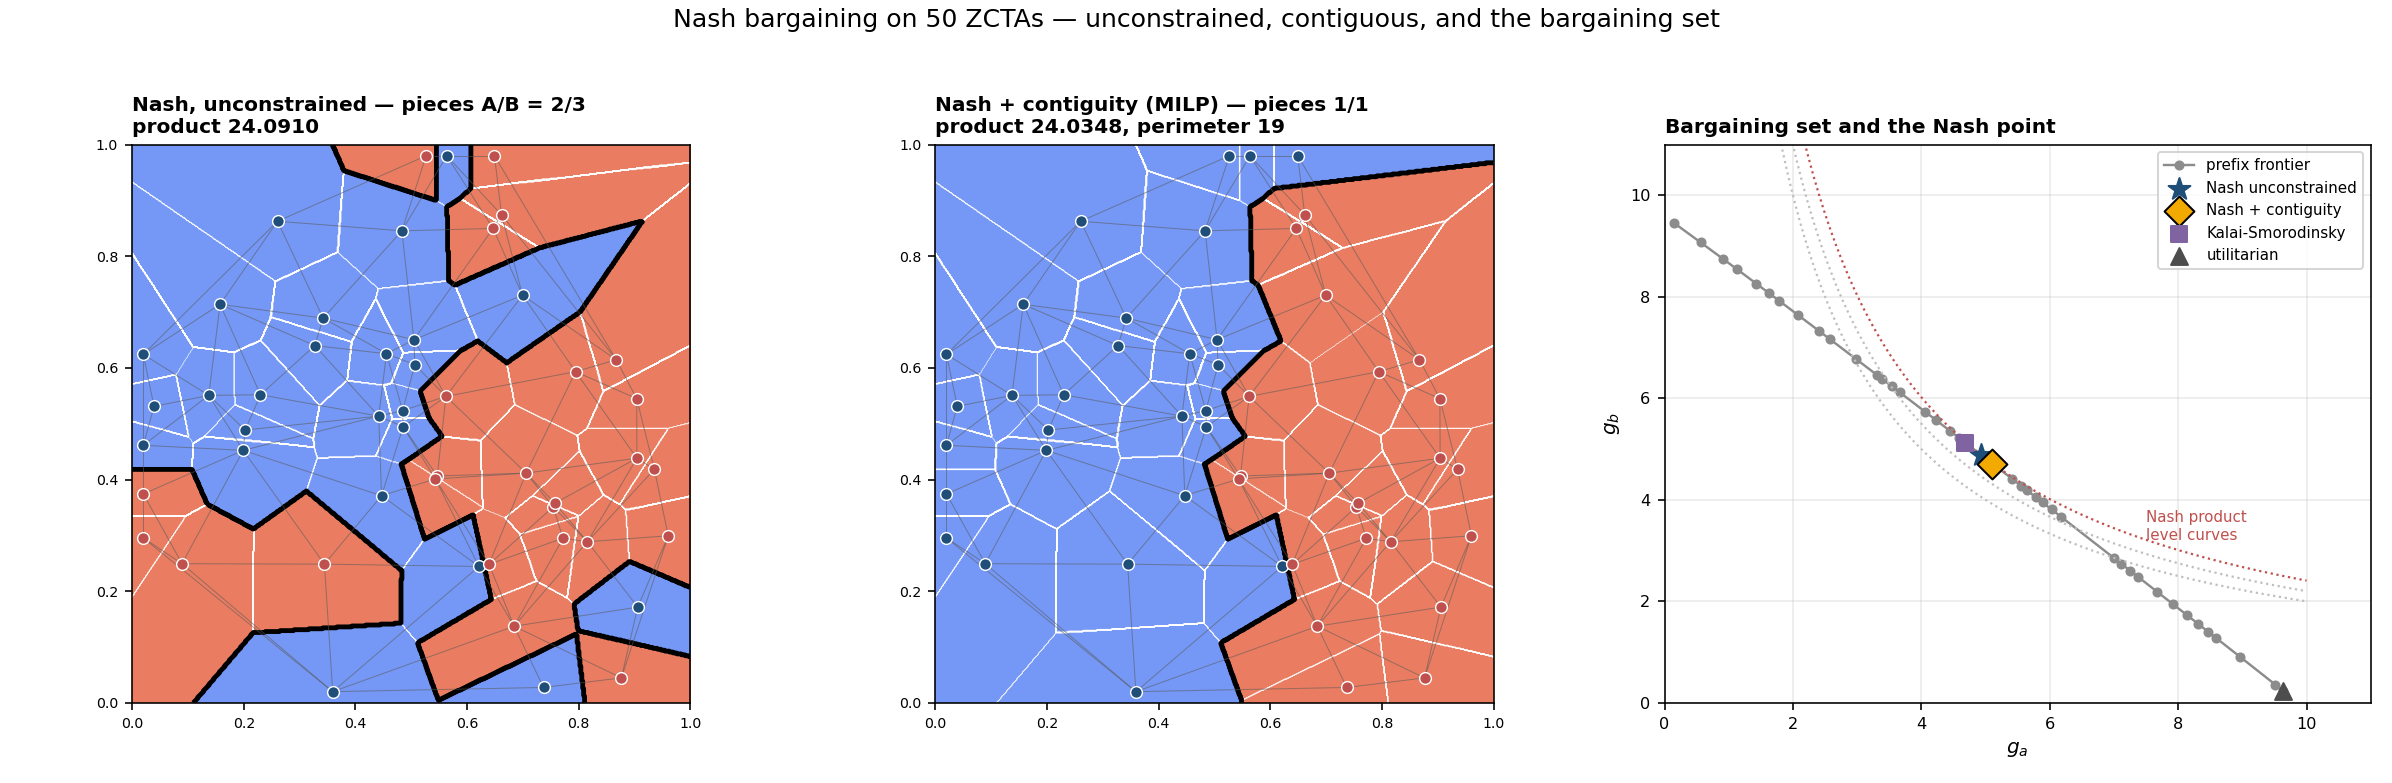
\includegraphics[width=\textwidth]{zip50_nash_milp.png}
\caption{Left: unconstrained Nash with the Rook adjacency overlaid; each wholesaler
holds a stray single-zip island. Centre: the contiguous MILP solution. Right: the
bargaining set --- grey points are the prefix frontier, dotted curves are level sets of
$g_ag_b$, and the Nash point is where the highest attainable level curve touches the
frontier. The utilitarian corner leaves $b$ with $0.24$.}\end{figure}

\section{Contestability}\label{sec:contest}
Where are the hard decisions? Two components, multiplied.

\paragraph{Stake.} Misassigning zip $z$ moves the bargaining product by, to first order,
\begin{equation}
\text{stake}_z=\frac{u_a(z)}{g_a}+\frac{u_b(z)}{g_b},
\end{equation}
the relative swing in $\log g_ag_b$. On the instance it ranged over
$[0.0336,\ 0.3556]$.

\paragraph{Doubt.} The flip rate $2\min(p,1-p)$ under uncertainty. Sweeping
$\theta\in[0.20,0.60]$ and $\lambda\in[0.10,0.50]$ moves few zips; perturbing the
\emph{data} by $10\%$ on sales and $6\%$ on opportunity moves $34$ of $50$.

\begin{resultbox}
Parameter uncertainty is nearly irrelevant here; data uncertainty dominates. Getting
$A_z$ and $B_z$ right matters more than settling $\lambda$.
\end{resultbox}

\begin{center}\begin{tabular}{lrrrl}\toprule
rank & zip & stake & doubt & quadrant\\ \midrule
1 & 32 & $0.3387$ & $0.362$ & adjudicate\\
2 & 22 & $0.1378$ & $0.792$ & adjudicate\\
3 & 19 & $0.1028$ & $0.873$ & adjudicate\\
4 & 28 & $0.0882$ & $0.915$ & coin-flip\\
5 & 10 & $0.0597$ & $0.992$ & coin-flip\\
\bottomrule\end{tabular}\end{center}

\noindent Four zips fall in the adjudicate quadrant; the top five carry $52\%$ of total
contestability. Zip $32$ carries by far the largest stake and moderate doubt, so it is
both the biggest and the most genuinely open question --- unlike under an equalising
criterion, where it registered as large but settled.

\begin{figure}[H]\centering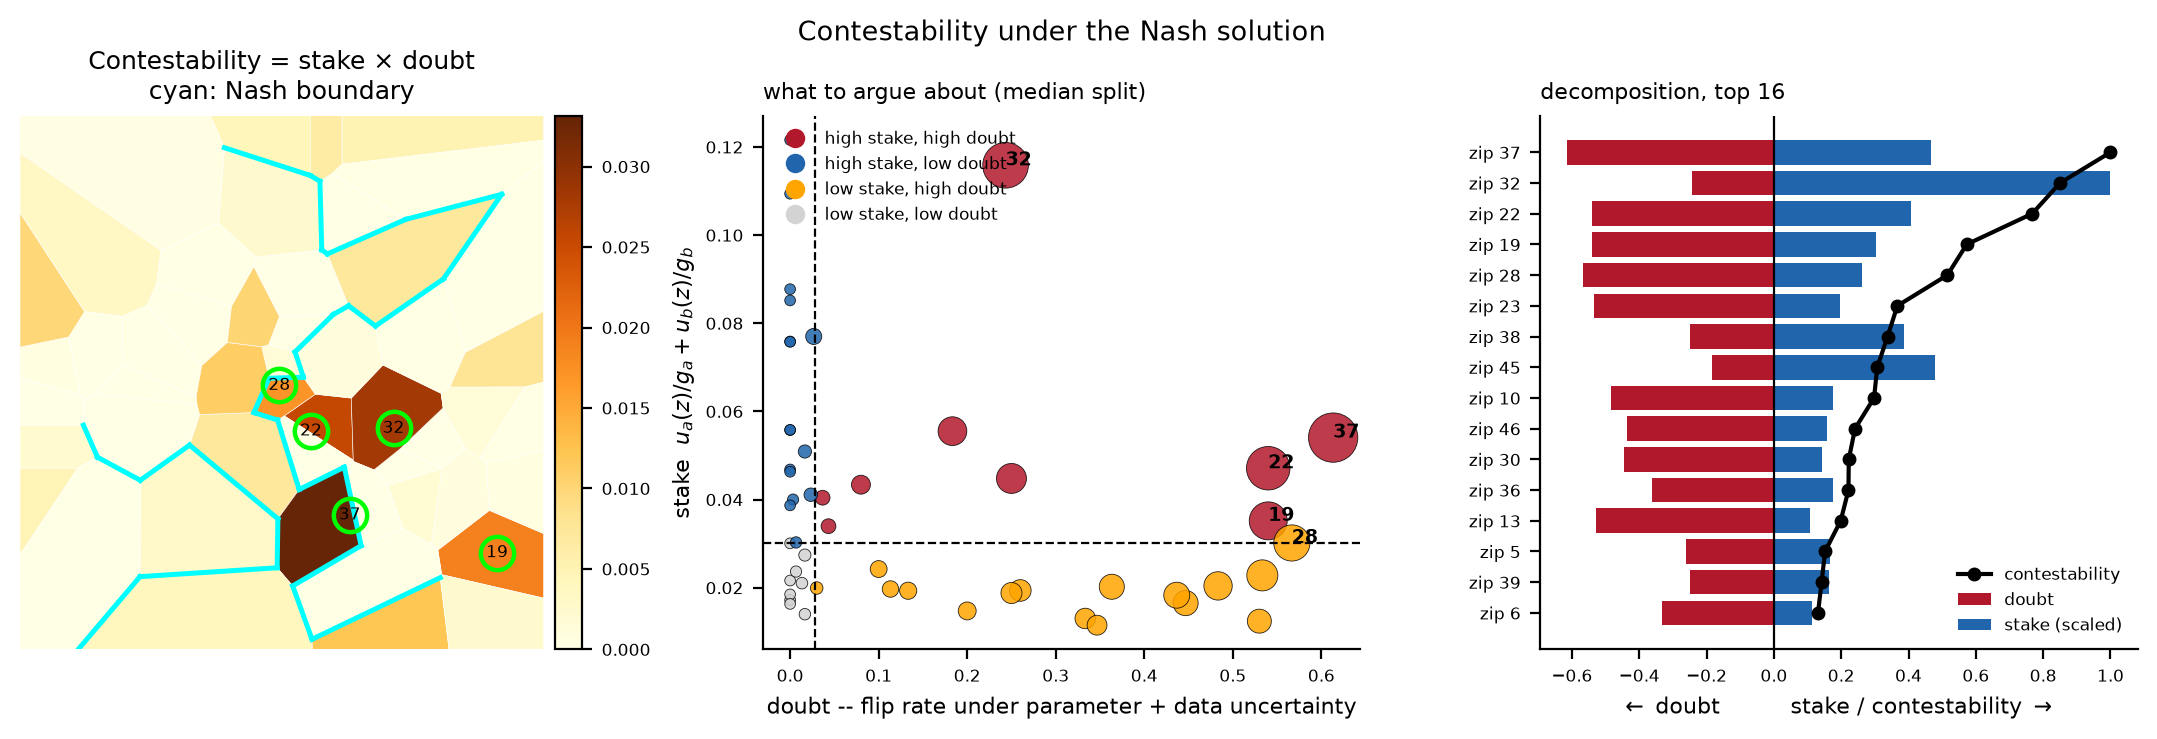
\includegraphics[width=\textwidth]{nash_contestability.png}
\caption{Contestability as stake $\times$ doubt. Left: mapped, Nash boundary in cyan,
top five ringed. Centre: the $2\times2$. Right: decomposition of the top sixteen.}
\end{figure}

\section{Exact parameter breakpoints}\label{sec:breaks}
Write $P_z=A_z+\theta B_z$, $Q_z=B_z+\theta A_z$, so $u_a(z)=(1-\lambda)P_z+\lambda M_z$.
Zips $i,j$ exchange places in the ratio order exactly when
\begin{equation}
(1-\lambda)K_{ij}+\lambda L_{ij}=0
\ \Longrightarrow\
\lambda^\star_{ij}=\frac{K_{ij}}{K_{ij}-L_{ij}},
\qquad
\begin{aligned}
K_{ij}&=P_iQ_j-P_jQ_i,\\
L_{ij}&=P_iM_j-P_jM_i+Q_jM_i-Q_iM_j .
\end{aligned}
\end{equation}
One explicit expression per pair; in $\theta$ the condition is quadratic, hence also
closed form. On the instance the Nash allocation takes only \textbf{ten distinct values}
across $\lambda\in[0.02,0.90]$.

\begin{resultbox}
$\lambda=0.30$ sits inside a flat interval from $0.265$ to $0.506$: anyone who believes
a dollar of untapped opportunity is worth between roughly $27$ and $50$ cents of booked
production obtains the same map. Nearly all sensitivity is crowded below
$\lambda\approx0.14$.
\end{resultbox}

\noindent This is a stronger instrument than a local derivative: rather than reporting
$dk/d\lambda$, one states the complete set of possible answers and exactly which belief
produces each.

\section{Opportunity balance}\label{sec:opp}
Before the merger both wholesalers covered the whole market, each with access to
$M=40$ at penetrations of $7.5\%$ and $4.5\%$. The honest framing is that both end with
roughly half of what they had. Under Nash, $M_a=21.23$ ($53.1\%$) against $M_b=18.77$,
an imbalance of $6.1\%$.

\begin{resultbox}
\textbf{$\lambda$ is the opportunity-balance dial.} The headroom term places most of the
weight on opportunity at moderate $\lambda$, so the criterion balances market size
without being asked to. Imbalance falls monotonically from $19.5\%$ at $\lambda=0.02$ to
about $1\%$ at $\lambda=0.70$. ``How much should untapped opportunity count?'' and
``should territories carry equal market size?'' are the same question.
\end{resultbox}

\noindent Imposing equal opportunity as a hard condition is possible but is a strong
position: with books of $3.0$ against $1.8$ it fully discounts the larger book. That is
a compensation-philosophy decision rather than a modelling one.

\section{Implementation and scope}\label{sec:impl}
\texttt{territory.py} operates on a \texttt{networkx} graph of ZCTAs with Rook adjacency
and attributes \texttt{rep\_a}, \texttt{rep\_b}, \texttt{A}, \texttt{B}, \texttt{M},
\texttt{state}: it validates headroom, builds the bipartite overlap graph of wholesaler
pairs and reports its component structure, solves each pair by prefix table, and writes
results back for mapping. \texttt{districting.py} adds the contiguous MILP, with
\texttt{solve\_contiguous\_nash} performing the $\varepsilon$-constraint sweep. Setting
\texttt{respect\_state=True} deletes cross-state edges before enforcing connectivity;
for life and annuity distribution this may bind harder than contiguity, since product
availability and producer appointments are state-scoped.

\paragraph{Not covered.} Capacity and travel constraints. Three or more wholesalers, for
which no threshold rule exists and the natural extension is leximin over each dense
component of the overlap graph. Estimation of $\theta$ from historical reassignments,
on which everything ultimately rests. At national scale, a solver with lazy-constraint
callbacks is preferable to re-solving from scratch each round.

\paragraph{Three checks on real data.}
\begin{enumerate}[leftmargin=*,itemsep=2pt]
\item $\mathrm{corr}(A_z,B_z)$ across zips --- whether the books overlap or separate,
and hence how contested the exercise is.
\item Connected components of the allocation on the true adjacency graph --- pricing
contiguity rather than assuming it.
\item Measurement error on $A_z,B_z,M_z$ --- since data uncertainty, not parameter
uncertainty, sets which zips need adjudication.
\end{enumerate}

\appendix
\section{Other solution concepts}\label{app:other}
Selecting each criterion directly over the fifty-one prefixes of the instance in
Section~\ref{sec:instance}:

\begin{center}\begin{tabular}{lrrrrrr}\toprule
\textbf{criterion} & $k$ & $g_a$ & $g_b$ & $g_ag_b$ & $\min(g)$ & $|g_a/\Amax-g_b/\Bmax|$\\
\midrule
\textbf{Nash} & $25$ & $4.9360$ & $4.8807$ & $\mathbf{24.091}$ & $4.8807$ & $0.0286$\\
equal gain & $25$ & $4.9360$ & $4.8807$ & $24.091$ & $4.8807$ & $0.0286$\\
egalitarian & $25$ & $4.9360$ & $4.8807$ & $24.091$ & $4.8807$ & $0.0286$\\
Kalai--Smorodinsky & $24$ & $4.6807$ & $5.1301$ & $24.012$ & $4.6807$ & $0.0137$\\
equal opportunity & $22$ & $4.4423$ & $5.3628$ & $23.823$ & $4.4423$ & $0.0532$\\
utilitarian & $46$ & $9.6330$ & $0.2395$ & $2.307$ & $0.2395$ & $0.8107$\\
\bottomrule\end{tabular}\end{center}

\noindent Nash, equal gain and the egalitarian criterion coincide. Kalai--Smorodinsky
differs substantively rather than by artefact: it equalises \emph{fractions} of
attainable gain, and $\Bmax=12.30$ exceeds $\Amax=11.60$ precisely because $b$ brought
the smaller book and has the lower baseline to clear. KS therefore awards more absolute
gain to the wholesaler who brought less production --- defensible in principle, awkward
to deliver. The utilitarian row shows what fairness buys: unconstrained, $a$ takes $46$
zips and leaves $b$ a gain of $0.24$.

\paragraph{Equalisation can destroy value.} Minimising a difference is not a monotone
objective, and the unconstrained equalising MILP illustrates the hazard: it reached a KS
gap of $0.000161$ at $82.1\%$ of attainable welfare, against $85.8\%$ for the best
prefix. The remedy is a welfare floor $g_a+g_b\ge\kappa\max_S(g_a+g_b)$, whose
right-hand side is available in closed form because the utilitarian optimum is the
prefix $\{z:u_a(z)>u_b(z)\}$. Nash needs no such guard.

\section{The prefix heuristic}\label{app:prefix}
Section~\ref{sec:nash} solves \eqref{eq:nashcriterion} exactly by outer approximation.
This appendix records a fast, solver-free alternative --- a sanity check and a preview,
not a substitute --- and the extent to which it can be trusted.

\subsection{Definition, and exactness for the utilitarian criterion only}
Define the utility ratio
\begin{equation}
r_z=\frac{u_a(z)}{u_b(z)},
\end{equation}
the rate at which utility transfers between the wholesalers when zip $z$ changes hands.

\begin{resultbox}
\begin{proposition}[Prefix heuristic]\label{prop:prefix}
Order the zips so that $r_{(1)}\ge\dots\ge r_{(n)}$ and write $P_k=\{(1),\dots,(k)\}$.
Then the utilitarian optimum is exactly $P_k$ with $k=|\{z:r_z>1\}|$, and
$\arg\max_k g_a[k]g_b[k]$ is a fast approximation to the Nash optimum.
\end{proposition}
\end{resultbox}

\noindent The utilitarian claim is exact: the objective is
$\sum_{z\in S}(u_a(z)-u_b(z))+\text{const}$, maximised by taking every zip with
$u_a>u_b$. The Nash claim is not. The usual argument --- at an optimum every included
zip satisfies $u_a(z)/g_a\ge u_b(z)/g_b$, a threshold on $r_z$ --- is \emph{marginal},
treating $g_a,g_b$ as fixed while a zip moves. Discretely they jump by a finite amount,
so the threshold characterisation is only asymptotically valid.

\begin{warnbox}
\textbf{The prefix rule is an approximation, and it is wrong about half the time.}
Against exhaustive enumeration over $200$ random instances per size:

\begin{center}
\begin{tabular}{crrr}
\toprule
$n$ & prefix optimal & mean shortfall & worst shortfall\\
\midrule
$6$ & $40.0\%$ & $3.91\%$ & $53.9\%$\\
$10$ & $47.5\%$ & $1.17\%$ & $13.9\%$\\
$14$ & $45.0\%$ & $0.57\%$ & $10.7\%$\\
\bottomrule
\end{tabular}
\qquad
\begin{tabular}{cr}
\toprule
$n$ & shortfall vs.\ local optimum\\
\midrule
$20$ & $0.16\%$\\
$50$ & $0.02\%$\\
$100$ & $0.002\%$\\
$400$ & $0.0009\%$\\
\bottomrule
\end{tabular}
\end{center}

\noindent The error vanishes as the discretisation refines, because the jumps shrink
relative to the gains. At realistic sizes it is far below the uncertainty in $\theta$
or in the sales data --- but it is not zero, and the rule should be described as a
heuristic, never substituted for Section~\ref{sec:nash}'s exact method where a
certificate matters.
\end{warnbox}

\subsection{Where it fails on other criteria}
Proposition~\ref{prop:prefix} covers Nash and the utilitarian criterion. It does not
extend to criteria that minimise a \emph{distance}, for which an off-frontier subset can
hit the target more precisely. Over $400{,}000$ random subsets of the worked instance:

\begin{center}\begin{tabular}{lrrl}\toprule
criterion & best prefix & best random subset & \\ \midrule
utilitarian $\max g_a+g_b$ & $32.983$ & $32.894$ & prefix holds\\
Nash $\max g_ag_b$ & $210.253$ & $201.896$ & prefix holds\\
egalitarian $\max\min(g)$ & $13.382$ & $14.096$ & \textbf{violated}\\
equal gain $\min|g_a-g_b|$ & $2.3287$ & $0.0001$ & \textbf{violated}\\
Kalai--Smorodinsky & $0.02240$ & $0.000004$ & \textbf{violated}\\
\bottomrule\end{tabular}\end{center}

\noindent The prefix table therefore remains exact for Nash, and is a fast restriction
for the others --- one with the merit of staying on a family of allocations ordered by
exchange rate.

\section{The mixture-quantile shortcut}\label{app:mixture}
For the \emph{equalisation} criteria the continuum analysis yields an appealing
shortcut. Collecting \eqref{eq:gains} under $g_a=g_b$ gives
\begin{equation}
\Phi(S)=q,\qquad
\Phi(S)=\frac{\Lambda\sum_{z\in S}(A_z+B_z)+2\lambda\sum_{z\in S}M_z}{D},
\qquad q=\frac{\Sa(1+c_2)-\lambda\Sb+\lambda M}{D},
\end{equation}
with $\Lambda=c_1+c_2$ and $D=\Lambda(\Sa+\Sb)+2\lambda M$: accumulate mixture mass
along the ratio order and cut where it crosses $q$. Kalai--Smorodinsky takes the same
form with weights $K_a=\Sa(\Bmax c_1+\Amax c_2)$, $K_b=\Sb(\Bmax c_2+\Amax c_1)$,
$K_M=\lambda M(\Amax+\Bmax)$ and level $q_{KS}=(\Amax\Bmax+\Bmax\Sa)/K$.

\begin{warnbox}
On a continuum this is exact. On discrete data it is off by one zip: $q$ is a continuum
target while the cumulative mass \emph{jumps}, so truncation need not give the nearer
prefix. With $q_{KS}=0.523326$ the crossing falls between $k=24$ (mass $0.517624$) and
$k=25$ ($0.535206$). On the equal-gain criterion the same truncation yields a gap of
$0.449$ where $k=25$ gives $0.055$.
\end{warnbox}

\noindent The mixture form remains valuable as \emph{theory} --- it makes $q$
interpretable, yields closed-form comparative statics, and reveals that $\lambda$
governs the weight on opportunity (Section~\ref{sec:opp}) --- but it is the wrong
algorithm for discrete data, and it does not arise for Nash at all.
\end{document}
